% !TEX program = xelatex

\documentclass[a4paper,11pt]{article}
\usepackage[margin=1in]{geometry}

\usepackage{fontspec}
\defaultfontfeatures{Numbers={OldStyle,Monospaced}}
\usepackage{newcomputermodern}
\setmonofont{Latin Modern Mono Light}
\usepackage{graphicx}
\usepackage{microtype}

\usepackage[ngerman]{babel}

\usepackage{tikz}
\usetikzlibrary{calc}
\usetikzlibrary{patterns}
\usetikzlibrary{shapes.geometric}
\pagenumbering{gobble} % No page numbers

\setsansfont[LetterSpace=8]{QTFuture}
\usepackage{enumitem}
\usepackage{booktabs}
\usepackage{siunitx}
\usepackage{float}
\usepackage{multicol}
\usepackage[hidelinks]{hyperref}
\usepackage[ngerman]{cleveref}
\usepackage{qrcode}

\renewcommand{\arraystretch}{1.25}
\setlength\parindent{0pt}

% \usepackage{fontawesome5}\newcommand\singlecup{\faCoffee}
\newcommand\singlecup{%
    \begin{tikzpicture}[line width=0.17ex,scale=0.7]
        \draw (-1.35ex,0ex) to[out=-45,in=180] (-0.8ex,-0.3ex) -- (0.8ex,-0.3ex) to[out=0,in=-135] (1.35ex,0ex);
        \fill (-0.92ex,1.5ex) -- (-0.92ex,0.5ex) to[out=270,in=180] (-0.3ex,-0.3ex) -- (0.3ex,-0.3ex) to[out=0,in=270] (0.92ex,0.5ex) -- (0.92ex,1.5ex) node (tr) {};
        \draw ($(tr.center) + (0,-0.15ex)$) to[out=0,in=90] ++(0.39ex,-0.3ex) to[out=270,in=0] ++(-0.39ex,-0.3ex);
    \end{tikzpicture}
}
\newcommand{\coffeecup}{\smash{\raisebox{0.6ex}{\singlecup}\hspace{-0.95em}\singlecup}}
\newcommand{\kettle}[1]{
    \smash{
        \begin{tikzpicture}[line width=0.2ex,scale=0.6,baseline=-0.5ex]
            \draw[semithick] (-1.7ex,2.1ex) -- (-1.3ex,1.7ex) -- (-1.3ex,-1.2ex) to[out=270,in=180] (-1.0ex,-1.5ex) -- (1.2ex,-1.5ex) to[out=0,in=270] (1.5ex,-1.2ex) -- (1.5ex,2.1ex) -- (1.7ex,2.1ex) to[out=0,in=90] (2.0ex,1.8ex) -- (2.0ex,-0.5ex) to[out=270,in=0] (1.7ex,-0.8ex) -- (1.5ex,-0.8ex);
            \foreach \y in {1,...,#1} { \node[fill,inner sep=0,rounded corners=0.1ex,minimum width=1.32ex,minimum height=0.35ex] at (0.1ex,{0.8ex*\y-1.67ex}) {}; }
        \end{tikzpicture}
    }
}

\begin{document}%
\begin{center}%
    KAFFEEMASCHINENGEBRAUCHSANWEISUNG\\
    Melitta 192 \textsc{a}1 $\cdot$ fmi
\end{center}
\begin{enumerate}[label={\textsc{schritt \arabic*:}},leftmargin=5.4em]
    \item Gegebenenfalls den alten Kaffeefilter samt Inhalt entsorgen.
    \item Gewünschte Menge Kaffee am Volumenkontrollrad (2) einstellen:

        \begin{tabular}{@{}rl@{}}
            \coffeecup:                          & Eine Tasse Kaffee.                                 \\
            \kettle1/\kettle2/\kettle3/\kettle4: & Eine viertel/halbe/dreiviertel/ganze Kanne Kaffee.
        \end{tabular}
    \item Neuen Filter einlegen.
    \item Kaffeepulver in den Filter legen.
        Referenzmengen richten sich nach \Cref{tab:mengen}.
    \item Kaffeemaschine durch Hauptschalter (5) aktivieren.\footnote{Vorsicht: Dies aktiviert auch die Heizplatte unter der Kanne.}
    \item Durch kurzes Bedienen des Aktivierungsschalters (3) Kaffee kochen.
    \item Auf Fertigstellungsleuchte (1) warten.
    \item Kaffeemaschine durch Hauptschalter (5) deaktivieren.
\end{enumerate}

\begin{center}
    VERHALTENSREGELN
\end{center}
\begin{itemize}[leftmargin=0em]
    % \item Kakao im Kaffee durch Verwendung von beispielsweise Klebezetteln kommunizieren.
    \item Kaffeekanne nach Leerung reinigen.
    \item Wer Kaffee macht, bekommt \emph{nie} die erste Tasse.
    \item Wer nicht für Kaffee bezahlt, ist doof.
\end{itemize}

\vfill

\begin{figure}[H]
    \centering
    \begin{tikzpicture}[outer sep=0]
        % Background Lines
        \foreach \y in {-0.5,-0.4,...,0.55}{ \draw[thick] (0,\y) -- (12,\y); }
        % Service Light
        \fill[white] (1.5,0) circle (0.45) node[outer sep=2mm] (OrangeLight) {};
        \draw[thick, pattern=crosshatch dots] (1.5,0) circle (0.35);
        \node at (1.5, 0.75) {\fontsize{5}{5}\selectfont\textsf{SERVICE}};
        % Green Light
        \fill[white] (2.5,0) circle (0.45) node[outer sep=7mm] (GreenLight) {};
        \draw[thick, pattern=crosshatch dots] (2.5,0) circle (0.35);
        % Knob
        \fill[white] (4.75,0) circle (1) node[outer sep=8mm] (Knob) {};
        \draw[thick] (4.75,0) circle (0.7);
        \draw[ultra thick] ($(4.75,0) + 0.7*({sin(-60)},{cos(-60)})$) -- (4.75, 0); % indicator
        \draw[fill=white] (4.75,0) circle (0.55);
        \draw (4.75,0) circle (0.45);
        \foreach \theta in {0,18,...,360} { \node[ellipse,fill,inner sep=0,minimum width=3,rotate=-\theta] at ($(4.75,0) + 0.54*({sin(\theta)},{cos(\theta)})$) {}; }
        % Knob UI
        \draw[thick,line cap=round] ($(4.75,0) + 0.85*({sin(-60)},{cos(-60)})$) node[circle,fill,inner sep=0.0375cm] {} -- ++(0,0.25) -- ++(-0.3,0.2);
        \node[anchor=base] at (3.55,1.08) {\footnotesize\coffeecup};
        \draw[thick,line cap=round] ($(4.75,0) + 0.85*({sin(-30)},{cos(-30)})$) node[circle,fill,inner sep=0.0375cm] {};
        \node[anchor=base] at (4.15,1.08) {\footnotesize\kettle{1}~};
        \draw[thick,line cap=round] ($(4.75,0) + 0.85*({sin(  0)},{cos(  0)})$) node[circle,fill,inner sep=0.0375cm] {};
        \node[anchor=base] at (4.75,1.08) {\footnotesize\kettle{2}~};
        \draw[thick,line cap=round] ($(4.75,0) + 0.85*({sin( 30)},{cos( 30)})$) node[circle,fill,inner sep=0.0375cm] {};
        \node[anchor=base] at (5.35,1.08) {\footnotesize\kettle{3}~};
        \draw[thick,line cap=round] ($(4.75,0) + 0.85*({sin( 60)},{cos( 60)})$) node[circle,fill,inner sep=0.0375cm] {} -- ++(0,0.25) -- ++(0.3,0.2);
        \node[anchor=base] at (5.95,1.08) {\footnotesize\kettle{4}~};
        % Buttons
        \fill[white] (6,-0.75) rectangle (11,0.75);
        \node [draw,inner sep=0,rounded corners=0.2cm,minimum width=1.3cm,minimum height=1.6cm,outer sep=2mm] (PowerSwitch) at (6.9,0) {};
        \node [draw,thick,inner sep=0,rounded corners=0.1cm,minimum width=1.0cm,minimum height=1.3cm] at (6.9,0) {\tiny\textsf{START}};
        %
        \node [draw,inner sep=0,rounded corners=0.2cm,minimum width=1.3cm,minimum height=1.6cm,outer sep=2mm] (TopBedSwitch) at (8.5,0) {};
        \node [draw,thick,inner sep=0,rounded corners=0.1cm,minimum width=1.0cm,minimum height=1.3cm] at (8.5,0) {};
        \node at (8.5, 0.3) {\scriptsize|};\node at (8.5,-0.3) {\scriptsize○};
        \fill (8.37,1.0) -- (8.63,1.0) -- (8.63,1.06) -- (8.6,1.06) -- (8.58,1.04) -- (8.42,1.04) -- (8.4,1.06) -- (8.37,1.06) --cycle;
        \foreach \x in {8.55,8.5,8.45} { \draw[semithick] (\x,1.08) -- ++(0,0.08) to[out=90,in=270] ++(0.017,0.08) to[out=90,in=270] ++(-0.025,0.07) to[out=90,in=250] ++(0.01,0.04); }
        %
        \node [draw,inner sep=0,rounded corners=0.2cm,minimum width=1.3cm,minimum height=1.6cm,outer sep=2mm] (MainSwitch) at (10.1,0) {};
        \node [draw,thick,inner sep=0,rounded corners=0.1cm,minimum width=1.0cm,minimum height=1.3cm] at (10.1,0) {};
        \node at (10.1, 0.3) {\scriptsize|};\node at (10.1,-0.3) {\scriptsize○};
        % Annotations
        \draw [<-,thick] (GreenLight.south)   -- ++(0mm,-1mm) to[out=270,in=90] ( 0,-1.75) node[below] {(1)};
        \draw [<-,thick] (Knob.south)         -- ++(0mm,-1mm) to[out=270,in=90] ( 3,-1.75) node[below] {(2)};
        \draw [<-,thick] (PowerSwitch.south)  -- ++(0mm,-1mm) to[out=270,in=90] ( 6,-1.75) node[below] {(3)};
        \draw [<-,thick] (TopBedSwitch.south) -- ++(0mm,-1mm) to[out=270,in=90] ( 9,-1.75) node[below] {(4)};
        \draw [<-,thick] (MainSwitch.south)   -- ++(0mm,-1mm) to[out=270,in=90] (12,-1.75) node[below] {(5)};
    \end{tikzpicture}
    \caption{
        Kontrollleiste der Kaffeemaschine.
        (1) Fertigstellungsleuchte, (2) Volumenkontrollrad, (3) Aktivierungsschalter, (4) Oberseitenheizplattenschalter und (5) Hauptschalter.
    }
\end{figure}

\begin{multicols}{2}%
    \begin{table}[H]%
        \centering%
        \caption{Referenzkaffeepulvermengen bezogen auf ,,Café Intención Ecológico``.}
        \label{tab:mengen}
        ~

        \begin{tabular}{@{}clc@{}}
            \toprule
            Symbol     & Bezeichnung       & {Menge /\textsc{üfmisl}} \\
            \midrule
            \coffeecup & Tasse             & 0,50                     \\
            \kettle1   & Viertel Kanne     & 1,25                     \\
            \kettle2   & Halbe Kanne       & 2,50                     \\
            \kettle3   & Dreiviertel Kanne & 3,75                     \\
            \kettle4   & Ganze Kanne       & 5,00                     \\
            \bottomrule
        \end{tabular}
    \end{table}
    \columnbreak

    \begin{figure}[H]
        \hfill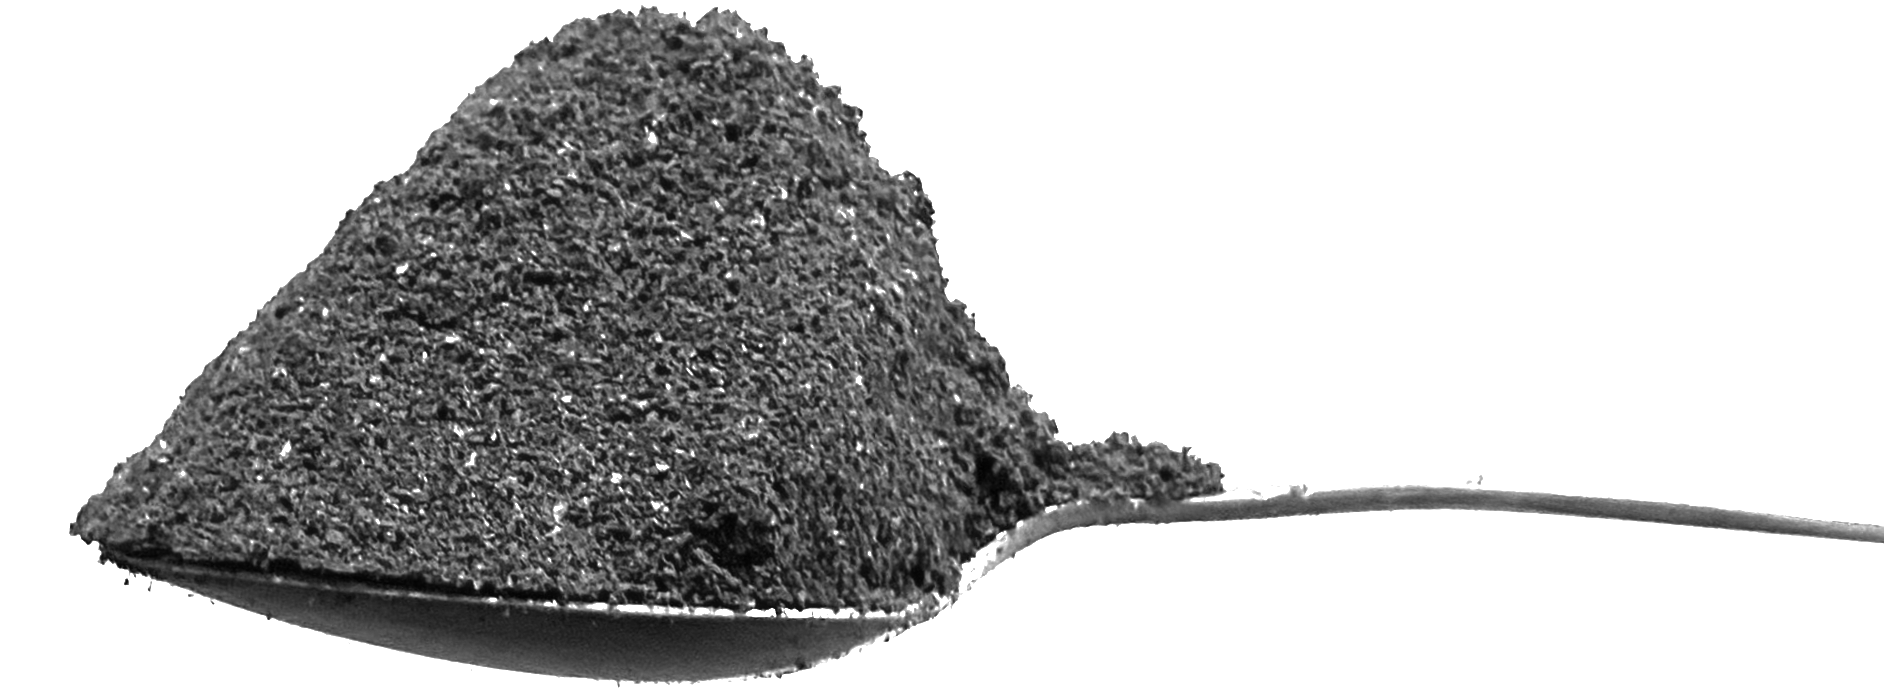
\includegraphics[width=0.7\linewidth]{uefmisl}
        \caption{Referenzmenge für die Normeinheit des \emph{Überfüllten Fachschaft Mathematik und Informatik Standardlöffels} (\textsc{üfmisl}).}
    \end{figure}

    \raisebox{0.4cm}{\qrcode[height=1cm]{github.com/Kamik423/fmi-coffee}}
    \begin{tikzpicture}[scale=0.75, baseline=(bottomtext.base)]
        \fill[gray] (0.25,-0.25) -- (0.25,0.25) -- (-1.125,0.25) to[out=180,in=90] (-1.25,0.125) -- (-1.25,-0.125) to[out=270,in=180] (-1.125,-0.25) --cycle;
        \node[inner sep=0,anchor=south,white] at (-0.5,-0.75ex) {\footnotesize{}License};
        \fill[black] (0.25,0.25) -- (0.25,-0.25) -- (1.125,-0.25) to[out=0,in=270] (1.25,-0.125) -- (1.25,0.125) to[out=90,in=0] (1.125,0.25) --cycle;
        \node[inner sep=0,anchor=south,white] at (0.75,-0.75ex) (mit) {\footnotesize\textsc{mit}\vphantom{L}};
        % link
        \node[inner sep=0,anchor=west] (bottomtext) at (-1.25,-0.5) {\footnotesize\url{github.com/Kamik423/fmi-coffee}};
        % LaTeX
        \node[inner sep=0,anchor=west] at (-1.25,0.5) {\footnotesize\LaTeX};
    \end{tikzpicture}
\end{multicols}
\end{document}